%Radio description
{\Large Radio Bands}
%Draw a sinewave with
%	{Initial Amplitude x.xxx}{Initial Time-width x.xxx}{Initial Number of cycles x}
%	{Second Amplitude x.xxx}{Second Time-width x.xxx}{Second Number of cycles x}
%	{Total repeats}
\newlength{\nAmplitude}		\newlength{\nAmplitudeNeg}
\newlength{\nTime}		\newlength{\nTimeTwo}		\newlength{\nTimeThree}		\newlength{\nTimeFour}
\newlength{\nSAmplitude}	\newlength{\nSAmplitudeNeg}
\newlength{\nSTime}		\newlength{\nSTimeTwo}		\newlength{\nSTimeThree}	\newlength{\nSTimeFour}
\newlength{\nTimeEnd}		\newlength{\nSTimeEnd}		\newlength{\nSTimeStart}
\newcommand{\sinewave}[7]{
	\setlength{\nAmplitude}{#1}
	\setlength{\nAmplitudeNeg}{\nAmplitude*-1}
	\setlength{\nTime}{#2}
	\setlength{\nTimeTwo}{\nTime*2}
	\setlength{\nTimeThree}{\nTime*3}
	\setlength{\nTimeFour}{\nTime*4}
	\setlength{\nTimeEnd}{\nTime*4*#3}
	\setlength{\nSAmplitude}{#4}
	\setlength{\nSAmplitudeNeg}{\nSAmplitude*-1}
	\setlength{\nSTime}{#5}
	\setlength{\nSTimeTwo}{\nSTime*2}
	\setlength{\nSTimeThree}{\nSTime*3}
	\setlength{\nSTimeFour}{\nSTime*4}
	\setlength{\nSTimeEnd}{\nTime*4*#3+\nSTime*4*#6}
	\multido{\dXTimePosition=0.000in+\nSTimeEnd}{#7}{
		\multido{\dXPosition=\dXTimePosition+\nTimeFour}{#3}{
			\rput(\dXPosition,0){
			\parabola(0.00,0)(\nTime,\nAmplitude)\parabola(\nTimeTwo,0)(\nTimeThree,\nAmplitudeNeg)
			}
		}
		\setlength{\nSTimeStart}{\dXTimePosition+\nTimeEnd}
		\multido{\dXPosition=\nSTimeStart+\nSTimeFour}{#6}{
			\rput(\dXPosition,0){
			\parabola(0.00,0)(\nSTime,\nSAmplitude)\parabola(\nSTimeTwo,0)(\nSTimeThree,\nSAmplitudeNeg)
			}
		}
	}
}
%

% None: f(x) = sin(20x)
% AM: f(x) = cos(.5x)∙sin(20∙x)
% FM: f(x) = cos(20∙x+15∙sin(x))


% Preamble:
% \pgfplotsset{width=7cm,compat=1.14}
% \begin{tikzpicture}
% \begin{axis}[
% hide x axis,
% hide y axis
% ]
% \addplot [red]{sin(deg(x))};
% \addplot [green]{cos(deg(x))};
% \end{axis}

% \begin{axis}[enlarge x limits=false]
% \addplot [red,samples=500] {sin(deg(x))};
% \addplot [orange,samples=7] {sin(deg(x))};
% \addplot [teal,const plot,samples=14]
% {sin(deg(x))};
% \end{axis}
% \end{tikzpicture}% <- eliminate space.
% \end{document}

% None: f(x) = sin(20x)
% AM: f(x) = cos(.5x)∙sin(20∙x)
% FM: f(x) = cos(20∙x+15∙sin(x))

\pgfplotsset{%
	axis line style={draw=none},
	tick style={draw=none},
	xticklabels=\empty,
	yticklabels=\empty,
	domain=0:3*pi,
	samples=1e3,
	width=2.3in,
	height=1in,
	xlabel shift=-8pt,
}

\begin{itemize}

%Country flags from here (using MIT license):
% https://github.com/stevenrskelton/flag-icon
% use inkscape to convert to eps which is smaller than using "convert"
%
%List of telecommunications regulatory bodies
% https://en.wikipedia.org/wiki/List_of_telecommunications_regulatory_bodies
%
\item {%
\setlength{\fboxsep}{0pt}%
\setlength{\fboxrule}{0.5pt}%
The radio spectrum (ELF to EHF) is populated by many more items than can be shown on this chart. Only a small sampling of the bands used around the world are shown. Each country has its own rules and regulations for allotting bands in this region. FCC \fbox{\includegraphics[width=0.15in]{tex/us.eps}}, CRTC \fbox{\includegraphics[width=0.15in]{tex/ca.eps}}, OFCOM \fbox{\includegraphics[width=0.15in]{tex/gb.eps}}, BNA  \fbox{\includegraphics[width=0.15in]{tex/de.eps}}, CII  \fbox{\includegraphics[width=0.15in]{tex/cn.eps}}...
}%
\item Communication by EMR is done by modulating the carrier waveform:

\begin{tabular}{ccc}%
\begin{tikzpicture} % No modulation
	\begin{axis}[smooth,grid=none,scale=1,xlabel={No modulation},line width=1pt,]
		\addplot[white, smooth,xlabel={No modulation},line join=round, line cap=round] {sin(x*20*180/pi)};
	\end{axis}
\end{tikzpicture}&
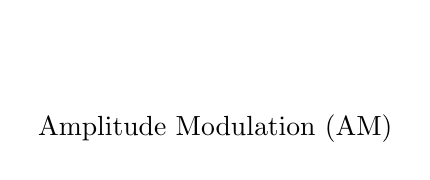
\begin{tikzpicture} %AM
	\begin{axis}[smooth,grid=none,scale=1,xlabel={Amplitude Modulation (AM)},line width=1pt,]
		%\addplot[white, smooth,line join=round, line cap=round] {sin(x*20*180/pi)*sin(x*1*180/pi)};
		\addplot[white, smooth,line join=round, line cap=round] {0.5*sin(x*20*180/pi)*(1+sin(x*1.7*180/pi))+8};

	\end{axis}
\end{tikzpicture}&
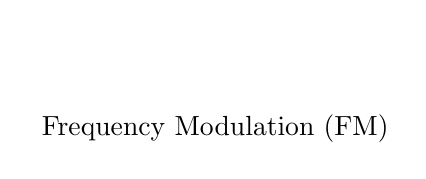
\begin{tikzpicture} % FM
	\begin{axis}[smooth,grid=none,scale=1,xlabel={Frequency Modulation (FM)},line width=1pt,]
		\addplot[white, smooth,line join=round, line cap=round] {sin((x*20 + 6*(sin(x*2*180/pi)))*180/pi)};
	\end{axis}
\end{tikzpicture}
\end{tabular}
%
% \item Not all references agree on the ULF band range, the HAARP range is used here.
%
\item {\bfseries RA}dio {\bfseries D}etecting {\bfseries A}nd {\bfseries R}anging (RADAR) uses microwaves to detect the distance and speed of objects.

\item {\bfseries C}itizens {\bfseries B}and Radio (CB) contains 40 stations between 26.965 - 27.405MHz %\hspace{0.02in}
{% CB Radio
  \definecolor{BoxColor}{rgb}{0.6,0.68,0.86}
  \psframebox[linestyle=none,framesep=1pt,fillcolor=BoxColor,linearc=0]{\black CB}
}.
%
 Schumann resonances are produced in the cavity between the Earth and the ionosphere \hspace{0.02in}%
 \psframebox[fillstyle=none,linestyle=none]{\psscalebox{0.7}{\blip{0,-.07}{S}}}%
 \hspace{0.02in}.
%
 Hydrogen gas emits radio band EMR at 21cm  \hspace{0.05in}%
 \psframebox[fillstyle=none,linestyle=none]{\psscalebox{0.7}{\blip{0,-.07}{H}}}%
 \hspace{0.02in}.
%
 Time / frequency standards shown as \psframebox[linestyle=none] {\rput(0.1in,0){\timestandard}} \hspace{0.1in}.
%
 Other individual frequencies are represented as icons:\vspace{0.1in}\\
\begin{tabular}{cp{1.4in}cp{1in}cp{1.7in}}
%
\psframebox[linestyle=none]{\submarine{0.02,.0}{xxHz}}\hspace{0.2in}\vspace{0.05in} & Submarine&
\psframebox[linestyle=none]{\rput(0.15,.05)\pager}&Pager&
\psframebox[linestyle=none]{\rput(0.05,.05){\psframebox[fillstyle=solid,fillcolor=Itinerant,linecolor=Itinerant,linearc=0,framesep=1pt]{\textcolor{Black}{GMRS}}}}&General Mobile Radio Service\\%
%
\psframebox[linestyle=none]{\rput(0.14,0.01){\psframebox[fillstyle=solid,fillcolor=green,linecolor=green,linearc=0]{\textcolor{Black}{xxm}}}}\hspace{.1in}\vspace{0.05in} & Ham / international&
\psframebox[linestyle=none]{\rput(0.14,.03){\weatherstation}\hspace{.03in}\vspace{0.08in}} & Weather&
\psframebox[linestyle=none]{\rput(0.15,.04){
	\psframe[linestyle=solid,linecolor=gray,fillstyle=solid,fillcolor=gray,linearc=0](-.2,-.08)(.2,.08)
	\psframe[hatchwidth=2pt, hatchsep=1.5pt,linestyle=solid,linecolor=yellow,fillstyle=hlines,hatchangle=45,hatchcolor=yellow,fillcolor=gray,linearc=0](-.2,-.08)(.2,.08)
	}
	\hspace{.2in}}\vspace{0.05in}
	& Short wave\\
%
%
\psframebox[linestyle=none]{\rput(0.11,.05){\psframebox[fillstyle=solid,fillcolor=Itinerant,linecolor=Itinerant,linearc=0,framesep=1pt]{\textcolor{Black}{FRS}}}}&Family Radio Service&
\psframebox[linestyle=none]{\rput(0.15,-0.1){\wirelessmic}}&Wireless Mic.&

\end{tabular}
\input{tex/morse.tex}
\end{itemize}
